% Phase-2 pixel digi morphing in the Alpaka clusterizer
% IIHE Tracker DPG meeting, 27 October 2026
% Internal: workshop figures (Indico 1707530) are CERN-restricted, so figures/ and the PDF stay out of git.
% Build: pdflatex phase2_morphing.tex (twice). Figures: ./fetch_figures.sh
\documentclass[aspectratio=169,10pt,xcolor=table]{beamer}
\usetheme{cmstalk}
\usepackage[utf8]{inputenc}
\usepackage[T1]{fontenc}
\usepackage{lmodern}
\usepackage{amsmath,amssymb}
\usepackage{booktabs,array}
\usepackage{graphicx}
\usepackage{hyperref}
\usepackage{listings}
\usetikzlibrary{arrows.meta,positioning,decorations.pathreplacing,calc}
\graphicspath{{figures/}}

% plot palette (same as the validation plots)
\definecolor{cbBlue}{HTML}{2A78D6}
\definecolor{cbOrange}{HTML}{EB6834}
\definecolor{cbGreen}{HTML}{1BAF7A}
\newcommand{\pos}[1]{\textcolor{cbBlue}{#1}}
\newcommand{\con}[1]{\textcolor{cbOrange}{#1}}
\newcommand{\HL}[1]{\textcolor{cbGreen!80!black}{#1}}
\newcommand{\src}[1]{\vfill{\hfill\scriptsize\color{cmsgrey}#1}}
\newcommand{\takeaway}[1]{\begin{center}\color{cmsblue}\textbf{#1}\end{center}}
\newcommand{\ttbar}{\ensuremath{\mathrm{t}\overline{\mathrm{t}}}}
\newcommand{\code}[1]{\texttt{\small #1}}
\newcommand{\footevent}{IIHE Tracker DPG, 27 Oct 2026}

\lstset{language=C++,
  basicstyle=\ttfamily\scriptsize,
  keywordstyle=\color{cmsblue}\bfseries,
  commentstyle=\color{cmsgrey}\itshape,
  stringstyle=\color{cbOrange!80!black},
  columns=fullflexible, keepspaces=true, showstringspaces=false,
  frame=single, rulecolor=\color{cmsblue!35}, backgroundcolor=\color{cmslight!45},
  xleftmargin=2pt, xrightmargin=2pt, aboveskip=4pt, belowskip=2pt,
  escapeinside={(*@}{@*)},
  morekeywords={uint32_t,int32_t,uint64_t,constexpr,auto}}
\newcommand{\hl}[1]{\colorbox{cbOrange!25}{#1}}

% clusters before 4 after 2 recovered [(6, 2), (6, 3), (9, 1), (9, 2)]
\newcommand{\morphA}{%
\draw[step=1,gray!35,very thin] (0,0) grid (9,15);
\fill[cbBlue] (3,3) rectangle ++(1,1);
\fill[cbBlue] (3,4) rectangle ++(1,1);
\fill[cbBlue] (7,4) rectangle ++(1,1);
\fill[cbBlue] (3,5) rectangle ++(1,1);
\fill[cbBlue] (2,7) rectangle ++(1,1);
\fill[cbBlue] (2,8) rectangle ++(1,1);
\fill[cbBlue] (1,10) rectangle ++(1,1);
\fill[cbBlue] (1,11) rectangle ++(1,1);
\fill[cbBlue] (1,12) rectangle ++(1,1);
\draw[gray!60] (0,0) rectangle (9,15);}
\newcommand{\morphB}{%
\draw[step=1,gray!35,very thin] (0,0) grid (9,15);
\fill[cbBlue] (3,3) rectangle ++(1,1);
\fill[cbBlue] (3,4) rectangle ++(1,1);
\fill[cbBlue] (7,4) rectangle ++(1,1);
\fill[cbBlue] (3,5) rectangle ++(1,1);
\fill[cbBlue] (2,7) rectangle ++(1,1);
\fill[cbBlue] (2,8) rectangle ++(1,1);
\fill[cbBlue] (1,10) rectangle ++(1,1);
\fill[cbBlue] (1,11) rectangle ++(1,1);
\fill[cbBlue] (1,12) rectangle ++(1,1);
\fill[cbOrange!45] (2,2) rectangle ++(1,1);
\fill[cbOrange!45] (3,2) rectangle ++(1,1);
\fill[cbOrange!45] (4,2) rectangle ++(1,1);
\fill[cbOrange!45] (2,3) rectangle ++(1,1);
\fill[cbOrange!45] (4,3) rectangle ++(1,1);
\fill[cbOrange!45] (6,3) rectangle ++(1,1);
\fill[cbOrange!45] (7,3) rectangle ++(1,1);
\fill[cbOrange!45] (8,3) rectangle ++(1,1);
\fill[cbOrange!45] (2,4) rectangle ++(1,1);
\fill[cbOrange!45] (4,4) rectangle ++(1,1);
\fill[cbOrange!45] (6,4) rectangle ++(1,1);
\fill[cbOrange!45] (8,4) rectangle ++(1,1);
\fill[cbOrange!45] (2,5) rectangle ++(1,1);
\fill[cbOrange!45] (4,5) rectangle ++(1,1);
\fill[cbOrange!45] (6,5) rectangle ++(1,1);
\fill[cbOrange!45] (7,5) rectangle ++(1,1);
\fill[cbOrange!45] (8,5) rectangle ++(1,1);
\fill[cbOrange!45] (1,6) rectangle ++(1,1);
\fill[cbOrange!45] (2,6) rectangle ++(1,1);
\fill[cbOrange!45] (3,6) rectangle ++(1,1);
\fill[cbOrange!45] (4,6) rectangle ++(1,1);
\fill[cbOrange!45] (1,7) rectangle ++(1,1);
\fill[cbOrange!45] (3,7) rectangle ++(1,1);
\fill[cbOrange!45] (1,8) rectangle ++(1,1);
\fill[cbOrange!45] (3,8) rectangle ++(1,1);
\fill[cbOrange!45] (0,9) rectangle ++(1,1);
\fill[cbOrange!45] (1,9) rectangle ++(1,1);
\fill[cbOrange!45] (2,9) rectangle ++(1,1);
\fill[cbOrange!45] (3,9) rectangle ++(1,1);
\fill[cbOrange!45] (0,10) rectangle ++(1,1);
\fill[cbOrange!45] (2,10) rectangle ++(1,1);
\fill[cbOrange!45] (0,11) rectangle ++(1,1);
\fill[cbOrange!45] (2,11) rectangle ++(1,1);
\fill[cbOrange!45] (0,12) rectangle ++(1,1);
\fill[cbOrange!45] (2,12) rectangle ++(1,1);
\fill[cbOrange!45] (0,13) rectangle ++(1,1);
\fill[cbOrange!45] (1,13) rectangle ++(1,1);
\fill[cbOrange!45] (2,13) rectangle ++(1,1);
\draw[gray!60] (0,0) rectangle (9,15);}
\newcommand{\morphC}{%
\draw[step=1,gray!35,very thin] (0,0) grid (9,15);
\fill[cbBlue] (3,3) rectangle ++(1,1);
\fill[cbBlue] (3,4) rectangle ++(1,1);
\fill[cbBlue] (7,4) rectangle ++(1,1);
\fill[cbBlue] (3,5) rectangle ++(1,1);
\fill[cbBlue] (2,7) rectangle ++(1,1);
\fill[cbBlue] (2,8) rectangle ++(1,1);
\fill[cbBlue] (1,10) rectangle ++(1,1);
\fill[cbBlue] (1,11) rectangle ++(1,1);
\fill[cbBlue] (1,12) rectangle ++(1,1);
\fill[cbGreen] (2,6) rectangle ++(1,1);
\fill[cbGreen] (3,6) rectangle ++(1,1);
\fill[cbGreen] (1,9) rectangle ++(1,1);
\fill[cbGreen] (2,9) rectangle ++(1,1);
\draw[gray!60] (0,0) rectangle (9,15);}
% dilated 38 recovered 4


\title[Phase-2 digi morphing]{Pixel digi morphing for Phase 2\\[0.2ex]{\large in the Alpaka pixel clusterizer}}
\author[C. Gupta]{Chirayu Gupta}
\institute{Vrije Universiteit Brussel (IIHE)}
\date{IIHE Tracker DPG meeting, 27 October 2026}

\begin{document}

% ===================================================================
\begin{frame}[plain]
  \vspace{1.6em}
  \begin{center}
    {\color{cmsblue}\Large\bfseries Pixel digi morphing for Phase 2}\\[0.6em]
    {\color{cmsblue}\large in the Alpaka pixel clusterizer}\\[2.0em]
    {\large\insertauthor}\\[0.8em]
    {\small\insertinstitute}\\[2.0em]
    {\small\color{cmsgrey}\insertdate}
  \end{center}
  \vfill
  \begin{tikzpicture}[remember picture,overlay]
    \fill[cmsblue] (current page.south west) rectangle ([yshift=0.5cm]current page.south east);
    \node[anchor=south,inner sep=0pt] at ([xshift=-1.6cm,yshift=0.9cm]current page.south)
      {\includegraphics[height=1.4cm]{CMSlogo_color.png}};
    \node[anchor=south west,inner sep=0pt] at ([xshift=-0.4cm,yshift=0.9cm]current page.south)
      {\includegraphics[height=1.4cm]{VUB_logo.png}};
    % the toy example: broken track (left) and after morphing (right)
    \begin{scope}[shift={([xshift=0.8cm,yshift=-1.2cm]current page.west)},scale=0.17]
      \morphA
    \end{scope}
    \begin{scope}[shift={([xshift=-2.35cm,yshift=-1.2cm]current page.east)},scale=0.17]
      \morphC
    \end{scope}
  \end{tikzpicture}
\end{frame}

% ===================================================================
\begin{frame}{Outline}
  \begin{columns}[T]
    \column{0.52\textwidth}
    \begin{enumerate}
      \item What we learned at the Tracker DPG workshop
      \item The Phase-2 Inner Tracker modules and their sizes
      \item GPU basics: blocks, threads, shared memory
      \item How \code{FindClus} is launched for Phase 1 and Phase 2
      \item From Phase-1 morphing to Phase-2 morphing:\\ variable module sizes, 44-column strips
      \item The code
      \item Validation on PU200 \ttbar\ events
      \item Configuration, files changed, status
    \end{enumerate}
    \column{0.44\textwidth}
    \begin{block}{In one line}
      Same 1-bit bitmap morphing as Run 3, applied to \textbf{44-column strips} of each Phase-2 module,
      inside the \textbf{same 48\,KB} of shared memory.
    \end{block}
    \vspace{4pt}
    \small Branch \code{Chirayu18/cmssw:phase2-digimorphing}\\
    (2 commits on \code{CMSSW\_20\_1\_X}, no PR yet)
  \end{columns}
\end{frame}

% ===================================================================
\section{Tracker DPG workshop}
\begin{frame}{Why morphing: a Run-3 lesson that carries over to Phase 2}
  \begin{columns}[T]
    \column{0.56\textwidth}
    \includegraphics[width=\textwidth]{schulz_run3_timeline.png}
    {\scriptsize\color{cmsgrey} J.~Schulz, HLT tracking, Tracker DPG workshop, 16 Oct 2026, slide 4}
    \column{0.42\textwidth}
    \textbf{Run 3 (2025)}
    \begin{itemize}
      \item Degraded charge collection $\to$ \con{broken clusters}
      \item Fix: \pos{pixel digi morphing} in the HLT (Phase-1 GPU clusterizer)
    \end{itemize}
    \textbf{Phase 2} (M.~Magherini, IT calibration)
    \begin{itemize}
      \item After $1\times10^{16}$: 3D signal $\approx 5$\,ke vs $\approx 1$\,ke threshold
      \item Higher threshold $\to$ ``edge pixels lost, \con{clusters break}''
      \item Aug 2025 test beam already saw cluster splitting (S.~Dutta)
    \end{itemize}
  \end{columns}
  \takeaway{Phase 2 will need the same tool, and nothing in the Alpaka Phase-2 path had it.}
\end{frame}

\begin{frame}{What the workshop fixed for the design}
  \vspace{4pt}
  \begin{center}\small
  \begin{tabular}{@{}>{\raggedright\arraybackslash}p{0.21\textwidth}>{\raggedright\arraybackslash}p{0.42\textwidth}>{\raggedright\arraybackslash}p{0.32\textwidth}@{}}
    \toprule
    Who (talk) & Fact & Consequence for morphing \\
    \midrule
    A.~Bocci (Alpaka), asked in person & Phase-2 HLT kernels stay within \textbf{48\,KB static shared memory}, same as Run 3 & no whole-module bitmap \\
    N.~Bartosik (geometry) & T40: ROC = \textbf{672 rows $\times$ 216 columns} of 25$\times$100\,\textmu m; big pixels at chip seams & module size differs by module type \\
    G.~Mersi (data formats) & sensor $\neq$ chip grid: $r_s = 2r_c + (c_c \bmod 2)$, $c_s = \lfloor c_c/2\rfloor$ & morph in \textbf{sensor} coordinates (what the clusterizer gets) \\
    M.~Magherini (IT calib.) & TBPX L1 $\approx 2\times10^{-3}$ hits/pixel/BX & $\approx$290 digis per L1 module: sparse \\
    M.~Musich (HLT reco) & Phase-2 HLT clustering runs on sim digis; IT RAW unpacker end 2026 & validate on sim digis now \\
    J.~Schulz (HLT tracking) & \code{hltPhase2SiPixelClustersSoA} feeds CA, mkFit, CKF, LST & morphing reaches all HLT tracking \\
    \bottomrule
  \end{tabular}
  \end{center}
  \src{Tracker DPG workshop, 14--16 Oct 2026, indico.cern.ch/event/1707530 (CERN-restricted)}
\end{frame}

% ===================================================================
\section{Phase-2 pixels}
\begin{frame}{The Phase-2 Inner Tracker modules}
  \begin{columns}[T]
    \column{0.46\textwidth}
    \includegraphics[width=\textwidth]{bartosik_dual_quad.png}
    {\scriptsize\color{cmsgrey} N.~Bartosik, geometry, Tracker DPG workshop, slide 12 (T40)}
    \column{0.52\textwidth}
    \vspace{2pt}
    \begin{center}\small
    \begin{tabular}{@{}lrrr@{}}
      \toprule
      Module & rows $\times$ cols & pixels & 2 bitmaps \\
      \midrule
      Phase 1 (fixed) & 160 $\times$ 416 & 67k & 16.6\,KB \\
      \midrule
      \multicolumn{4}{@{}l}{\textit{Phase 2, measured in D128 geometry:}} \\
      TBPX L1 (1 chip) & 672 $\times$ 216 & 145k & 36\,KB \\
      dual (2 chips) & 672 $\times$ 434 & 292k & 73\,KB \\
      quad (4 chips) & 1354 $\times$ 434 & 588k & \con{149\,KB} \\
      \bottomrule
    \end{tabular}
    \end{center}
    \begin{itemize}\small
      \item Pixel 25\,\textmu m (row, $x$) $\times$ 100\,\textmu m (column, $y$)
      \item Big pixels = \textbf{one index} each $\to$ +2 rows/cols ($432\to434$, $1344\to1354$)
      \item Big-pixel $x$ pitch: 87.5 (Bartosik) vs 112\,\textmu m (Mersi), \textit{open}; irrelevant in index space
    \end{itemize}
  \end{columns}
  \takeaway{Three module sizes, all bigger than Phase 1: the size must be a run-time input.}
\end{frame}

\begin{frame}{Variable module size: what changes for the kernel}
  \begin{columns}[T]
    \column{0.48\textwidth}
    \textbf{Phase 1}: every module is 160 $\times$ 416
    \begin{itemize}
      \item bitmap layout is \code{constexpr}: 5 words/column, 2080 words
      \item edge rule uses fixed last row/column
    \end{itemize}
    \textbf{Phase 2}: size depends on the module
    \begin{itemize}
      \item read from \code{PixelTopology} in \code{beginRun}
      \item packed per morphing module: \code{rows<<16 | cols}
      \item kernel derives the layout from it:
    \end{itemize}
    \[
      W = \left\lceil \tfrac{\text{rows}}{32} \right\rceil, \qquad
      \text{mask} = 2^{\,\text{rows} \bmod 32} - 1
    \]
    {\small $W$ = words per column (21 for 672 rows, 43 for 1354); the mask removes the rows past the module in the last word.}
    \column{0.48\textwidth}
    \centering
    \begin{tikzpicture}[x=0.55cm,y=0.42cm,font=\footnotesize]
      % one column of the bitmap = W words of 32 rows
      \foreach \w/\lab in {0/word 0, 1/word 1, 3/word $W\!-\!1$} {
        \draw[fill=cmslight] (0,-\w) rectangle (6,-\w-0.8);
        \node[anchor=east] at (-0.1,-\w-0.4) {\lab};
      }
      \node at (3,-2.35) {$\vdots$};
      \fill[cbOrange!40] (4.2,-3) rectangle (6,-3.8);
      \node[font=\scriptsize,align=center] at (3.6,-4.4) {rows past the module: masked};
      \draw[decorate,decoration={brace,amplitude=4pt}] (0,0.1) -- node[above=4pt]{32 rows (bits)} (6,0.1);
      \node[font=\scriptsize] at (3,-5.4) {one column $y$ of the module};
      % column index direction
      \draw[-{Stealth},thick,cmsblue] (7,0) -- (7,-3.8) node[midway,right,align=left]{$x$\\ (row)};
    \end{tikzpicture}
  \end{columns}
\end{frame}

% ===================================================================
\section{GPU basics and the work division}
\begin{frame}{GPU basics: grid, blocks, threads, shared memory}
  \begin{columns}[T]
    \column{0.50\textwidth}
    \centering
    \begin{tikzpicture}[font=\footnotesize]
      % grid of blocks
      \foreach \i in {0,...,3} \foreach \j in {0,1}
        \draw[fill=cmslight] (\i*0.9,-\j*0.75) rectangle ++(0.75,0.6);
      \node[font=\scriptsize] at (0.375,0.3) {b0};
      \node[font=\scriptsize] at (1.275,0.3) {b1};
      \node at (4.0,-0.1) {$\cdots$};
      \node[anchor=south west,font=\small\bfseries,cmsblue] at (0,0.65) {grid of blocks};
      % zoom on one block of the bottom row
      \draw[thick,cmsblue,fill=cbBlue!30] (0,-0.75) rectangle (0.75,-0.15);
      \draw[cmsblue,dashed] (0,-0.75) -- (0,-1.6);
      \draw[cmsblue,dashed] (0.75,-0.75) -- (4.6,-1.6);
      \draw[thick,cmsblue,rounded corners] (0,-1.6) rectangle (4.6,-4.5);
      \node[anchor=north west,font=\scriptsize\bfseries,cmsblue] at (0,-1.6) {one block = runs on one SM};
      % warps
      \foreach \k in {0,1,2} {
        \foreach \t in {0,...,7} \draw[fill=cbBlue!60] (0.2+\t*0.18,-2.2-\k*0.4) rectangle ++(0.13,0.26);
        \node[anchor=west,font=\scriptsize] at (1.65,-2.07-\k*0.4) {warp \k: 32 threads, lockstep};
      }
      \node[font=\scriptsize,anchor=west] at (0.2,-3.25) {\ldots\ 12 warps = 384 threads};
      \draw[fill=cbOrange!30] (0.2,-4.35) rectangle (4.4,-3.55);
      \node[font=\scriptsize,align=center,text width=3.9cm] at (2.3,-3.95) {\textbf{shared memory} of the block, $\le$ 48\,KB};
    \end{tikzpicture}
    \column{0.48\textwidth}
    \begin{itemize}
      \item Kernel launch = \textbf{work division}: number of blocks $\times$ threads per block
      \item Blocks are independent; threads \emph{within} a block share memory and can \code{syncBlockThreads}
      \item \textbf{Shared memory}: on-chip, fast, per block\\ Run 3 and Phase-2 HLT budget: \textbf{48\,KB}
      \item \textbf{Registers}: per thread; they cap the block size\\
        T4: \code{FindClus} uses 143 registers $\to$ at most \textbf{384 threads} per block
      \item Alpaka: \code{independent\_group\_elements(acc, n)} = the block's threads stride over $n$ items
    \end{itemize}
  \end{columns}
  \takeaway{Everything one block needs for one module must fit in 48\,KB of shared memory.}
\end{frame}

\begin{frame}[fragile]{The \code{FindClus} work division: Phase 1 vs Phase 2}
  \begin{columns}[T]
    \column{0.49\textwidth}
    \textbf{Phase 1}: \textbf{64 blocks}, each loops over modules
    \begin{center}
    \begin{tikzpicture}[font=\scriptsize,x=0.42cm,y=0.42cm]
      \foreach \b in {0,1,2} {
        \node[draw,fill=cbBlue!25,minimum width=0.9cm,minimum height=0.32cm] (B\b) at (0,-\b*1.2) {block \b};
        \foreach \m [count=\n] in {\b,\b+64,\b+128} {
          \pgfmathtruncatemacro{\mm}{\m}
          \node[draw,fill=cmslight,minimum width=0.9cm,minimum height=0.32cm] at (2.2+\n*2.5,-\b*1.2) {mod \mm};
        }
        \draw[-{Stealth}] (B\b.east) -- ++(0.9,0);
        \node at (12.8,-\b*1.2) {$\cdots$};
      }
      \node at (0,-3.4) {$\vdots$};
    \end{tikzpicture}
    \end{center}
    \begin{itemize}\small
      \item fake pixels stored \textbf{per block}: $64 \times 2400$
    \end{itemize}
    \column{0.49\textwidth}
    \textbf{Phase 2}: \textbf{4000 blocks}, one per module
    \begin{center}
    \begin{tikzpicture}[font=\scriptsize,x=0.42cm,y=0.42cm]
      \foreach \b/\lab in {0/0,1/1,2/2} {
        \node[draw,fill=cbBlue!25,minimum width=0.9cm,minimum height=0.32cm] (C\b) at (0,-\b*1.2) {block \lab};
        \node[draw,fill=cmslight,minimum width=0.9cm,minimum height=0.32cm] (M\b) at (5,-\b*1.2) {mod \lab};
        \draw[-{Stealth}] (C\b.east) -- (M\b.west);
      }
      \node at (0,-3.4) {$\vdots$};
      \node[draw,fill=cbBlue!25,minimum width=0.9cm,minimum height=0.32cm] at (0,-4.6) {block 3999};
    \end{tikzpicture}
    \end{center}
    \begin{itemize}\small
      \item already so in master (\code{makePhase2ClustersAsync}), kept
      \item per-block fakes would be $4000\times1000$ slots: \con{18$\times$ more}
      \item instead: \textbf{per morphing module}, $216 \times 1000 \approx$ \pos{4.5\,MB}
    \end{itemize}
  \end{columns}
\begin{lstlisting}
// slot of this module in the sorted list of morphing modules (binary search), or -1
const int32_t morphingIndex = enableDigiMorphing ? morphingModuleIndex(rawModuleId, ...) : -1;
// Phase 1: fakes per block;  Phase 2: fakes per morphing module
const uint32_t firstFake = maxFakesInModule * (isPhase2 ? max(morphingIndex, 0) : block);
\end{lstlisting}
\end{frame}

% ===================================================================
\section{The algorithm}
\begin{frame}{Phase-1 morphing (Run 3): a closing on a 1-bit bitmap}
  \begin{columns}[T]
    \column{0.58\textwidth}
    \centering
    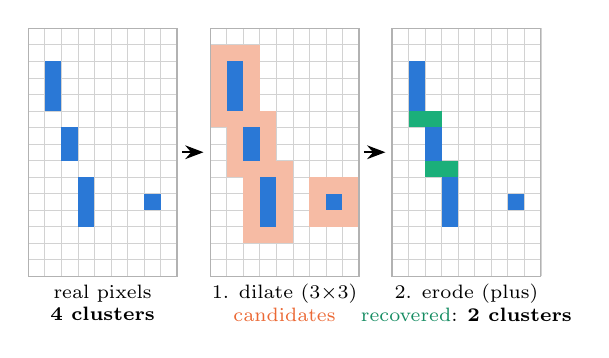
\begin{tikzpicture}[scale=0.21]
      \begin{scope}\morphA\end{scope}
      \node[font=\scriptsize,align=center] at (4.5,-1.6) {real pixels\\ \textbf{4 clusters}};
      \begin{scope}[shift={(11,0)}]\morphB\end{scope}
      \node[font=\scriptsize,align=center] at (15.5,-1.6) {1. dilate (3$\times$3)\\ \textcolor{cbOrange}{candidates}};
      \begin{scope}[shift={(22,0)}]\morphC\end{scope}
      \node[font=\scriptsize,align=center] at (26.5,-1.6) {2. erode (plus)\\ \textcolor{cbGreen!80!black}{recovered}: \textbf{2 clusters}};
      \draw[-{Stealth},thick] (9.3,7.5) -- (10.6,7.5);
      \draw[-{Stealth},thick] (20.3,7.5) -- (21.6,7.5);
    \end{tikzpicture}

    \vspace{4pt}
    \parbox{0.95\linewidth}{\centering\scriptsize Toy example computed with the kernel's rules: the track is joined,\\ the pixel 3 columns away is not.}
    \column{0.40\textwidth}
    \begin{itemize}
      \item \code{image}: 1 bit per pixel, 32 rows per word
      \item \textbf{dilate}: \code{temp} = empty pixels with any of the 8 neighbours set
      \item \textbf{erode}: keep a candidate if its 4 neighbours are all in \code{image} $\cup$ \code{temp}
      \item recovered (``fake'') pixels only \textbf{link} clusters; they are dropped before the output, no charge added
      \item edge rule: beyond a row edge counts as \emph{filled}, beyond a column edge as \emph{empty}
    \end{itemize}
  \end{columns}
  \takeaway{32 pixels per instruction: shifts, ORs and ANDs on whole words.}
\end{frame}

\begin{frame}{Why it cannot be ported as it is}
  \begin{columns}[T]
    \column{0.50\textwidth}
    \textbf{Shared memory of \code{FindClus}, Phase 2}
    \vspace{4pt}
    \begin{center}\small
    \begin{tabular}{@{}lr@{}}
      \toprule
      Item & bytes \\
      \midrule
      histogram \code{off} ($1001\times4$) & 4\,004 \\
      histogram \code{content} ($6000\times2$) & 12\,000 \\
      scalars, scan workspace, compiler & $\approx$\,3\,000 \\
      \midrule
      \textbf{already used} & $\approx$\,\textbf{19\,KB} \\
      \textbf{whole-module bitmaps, quad} & \con{\textbf{149\,KB}} \\
      \bottomrule
    \end{tabular}
    \end{center}
    \column{0.47\textwidth}
    Options considered
    \begin{itemize}
      \item \con{Whole-module bitmap in shared memory}: 3$\times$ over budget for a quad, 36\,KB even for L1
      \item \con{Bitmap in global memory}: $\sim$ 150\,KB per block, slow atomics
      \item \con{Sparse lookup in the column histogram}: no bitmap, but new logic to prove equal
      \item \pos{Same bitmap, one strip of columns at a time}: reuses the Phase-1 bit logic and \textbf{the Phase-1 buffers}
    \end{itemize}
  \end{columns}
  \takeaway{Keep the Run-3 algorithm, shrink the area it works on.}
\end{frame}

\begin{frame}{Strips of 44 columns with a 2-column halo}
  \centering
  \begin{tikzpicture}[x=0.024cm,y=0.8cm,font=\scriptsize]
    % TBPX L1 module 216 columns
    \node[anchor=east,align=right] at (-3,0.5) {TBPX L1\\ 672 $\times$ 216};
    \foreach \s/\e [count=\k] in {0/44,44/88,88/132,132/176,176/216} {
      \draw[fill=cmslight] (\s,0) rectangle (\e,1);
      \node at ({(\s+\e)/2},0.5) {\k};
    }
    \fill[cbOrange!45] (42,0) rectangle (44,1);
    \fill[cbOrange!45] (88,0) rectangle (90,1);
    \draw[very thick,cbOrange] (42,-0.08) rectangle (90,1.08);
    \draw[decorate,decoration={brace,amplitude=4pt,mirror}] (42,-0.15) -- node[below=4pt,align=center]{buffer: 48 columns = 2 + 44 + 2} (90,-0.15);
    % dual/quad 434 columns
    \begin{scope}[shift={(0,-2.1)}]
      \node[anchor=east,align=right] at (-3,0.5) {dual / quad\\ 672 or 1354 $\times$ 434};
      \foreach \k in {0,...,8} {
        \draw[fill=cmslight] (\k*44,0) rectangle ({(\k+1)*44},1);
        \node at ({\k*44+22},0.5) {\the\numexpr\k+1\relax};
      }
      \draw[fill=cmslight] (396,0) rectangle (434,1);
      \node at (415,0.5) {10};
    \end{scope}
  \end{tikzpicture}

  \vspace{6pt}
  \begin{columns}[T]
    \column{0.48\textwidth}
    \begin{itemize}
      \item Load the real pixels of 48 columns into \code{image} (from the column histogram, contiguous)
      \item Dilate the 46 inner columns, erode and \textbf{emit fakes for the 44 strip columns only}
      \item Halo columns outside the module stay empty (column edge rule)
    \end{itemize}
    \column{0.48\textwidth}
    \begin{itemize}
      \item \textbf{Skip} strips with no pixel within $\pm1$ column: one comparison of \code{hist.off}
      \item 5 strips for L1, 10 for 434-column modules
      \item Same answer as a whole-module bitmap \textbf{by construction} (shown on next slides)
    \end{itemize}
  \end{columns}
\end{frame}

\begin{frame}{Why 44 columns, and why a halo of 2}
  \begin{columns}[T]
    \column{0.48\textwidth}
    \textbf{44: the widest strip that fits the Phase-1 buffers}
    \[
      (\underbrace{S}_{\text{strip}} + 2\cdot\underbrace{2}_{\text{halo}})\times\underbrace{43}_{\lceil 1376/32\rceil} \;\le\; \underbrace{2080}_{\text{Phase-1 words}}
    \]
    \[
      S + 4 \le 48.4 \;\Rightarrow\; S = 44, \quad 48\times43 = 2064 \text{ words}
    \]
    \begin{itemize}\small
      \item 2080 = Phase-1 buffer size ($160/32 \times 416$)
      \item 1376 = 1354 rows rounded up to a word
      \item \pos{zero extra shared memory}: same two 8.3\,KB arrays
    \end{itemize}
    \column{0.50\textwidth}
    \textbf{Halo 2: erosion needs the dilation of the next column}
    \vspace{2pt}
    \begin{center}
    \begin{tikzpicture}[font=\scriptsize,x=1.3cm,y=0.75cm]
      \foreach \c/\lab/\col in {0/{$c$\\ last strip\\ column}/cmslight, 1/{$c+1$\\ halo 1}/cbOrange!25, 2/{$c+2$\\ halo 2}/cbOrange!25, 3/{$c+3$\\ not\\ loaded}/white} {
        \node[draw,fill=\col,minimum width=1.2cm,minimum height=1.0cm,text width=1.1cm,align=center] (K\c) at (\c,0) {\lab};
      }
      \draw[-{Stealth},thick,cbGreen!80!black] (K0.north) to[bend left=40] node[above,align=center]{erode $c$ reads\\ dilated $c+1$} (K1.north);
      \draw[-{Stealth},thick,cbBlue] (K1.south) to[bend right=40] node[below,align=center]{dilate $c+1$ reads\\ image $c+2$} (K2.south);
    \end{tikzpicture}
    \end{center}
    \begin{itemize}\small
      \item halo 1 would miss pixels at every strip edge
      \item \textbf{control}: halo = 1 fails in 4 of 5 morphing modules in the unit test
      \item the CPU \code{SiPixelDigiMorphing} has exactly this bug (next section)
    \end{itemize}
  \end{columns}
\end{frame}

\begin{frame}{Keeping the block size: fakes live inside the histogram}
  \begin{columns}[T]
    \column{0.50\textwidth}
    \textbf{Problem} (found on the T4, not on CPU)
    \begin{itemize}
      \item Phase 1 grows the histogram for fakes: $6000 + 2400$ entries $\to$ more threads per block
      \item For Phase 2 that gave 448 threads; at 143 registers the T4 allows 384
      \item \con{\code{cudaErrorLaunchOutOfResources}}
    \end{itemize}
    \textbf{Fix}
    \begin{itemize}
      \item in morphing modules: \textbf{5000 real + 1000 fake} entries $=6000$
      \item block size stays 384, \code{SimplePixelTopology.h} untouched
      \item max fakes seen in one module: 536
    \end{itemize}
    \column{0.47\textwidth}
    \textbf{Measured \code{FindClus} resources (sm\_75)}
    \vspace{4pt}
    \begin{center}\small
    \begin{tabular}{@{}lrr@{}}
      \toprule
      & Phase 1 & Phase 2 \\
      \midrule
      shared memory & 38\,200\,B & 35\,728\,B \\
      registers/thread & -- & 143 \\
      threads/block & -- & 384 \\
      \bottomrule
    \end{tabular}
    \end{center}
    {\small Phase 1 unchanged w.r.t.\ master. First attempt: 52\,624\,B, \con{over 48\,KB}: nvlink reserved the Phase-1 bitmaps in the Phase-2 kernel despite \code{if constexpr} $\to$ \pos{one pair of buffers declared for both phases.}}
  \end{columns}
  \takeaway{Measure on the GPU: both limits were invisible on the CPU backend.}
\end{frame}

% ===================================================================
\section{The code}
\begin{frame}[fragile]{Code 1: selecting the modules and their size (\code{SiPixelPhase2DigiToCluster.cc})}
\begin{lstlisting}
// beginRun: select the morphing modules from the geometry, and record their size
for (auto const* det : dets) {
  if (!GeomDetEnumerators::isInnerTracker(det->subDetector())) continue;
  DetId detId = det->geographicalId();
  if ((*@\hl{siPixelMorphing::skipDetId}@*)(&trackerTopology, detId, barrelRegions, endcapRegions)) continue;
  auto const& topology = dynamic_cast<PixelGeomDetUnit const&>(*det).specificTopology();
  const int nRows = topology.nrows(), nCols = topology.ncolumns();
  if (nRows > phase2Morphing::maxRows or nCols >= Phase2::clusterBinning)
    throw cms::Exception("Configuration") << "...";          // up to 1376 rows and 999 columns
  modules.emplace_back(detId.rawId(), (*@\hl{phase2Morphing::packSize(nRows, nCols)}@*));  // rows<<16 | cols
}
std::sort(modules.begin(), modules.end());     // sorted on the host: binary search on the device
// acquire(): both arrays are copied to the device once after each beginRun

// makePhase2ClustersAsync: same 4000-block launch as master; fakes only for morphing modules
auto fakes_d = SiPixelDigisSoACollection(queue, doMorphing ? nMorphingModules * maxFakes : 0);
\end{lstlisting}
  \begin{itemize}\small
    \item Phase 2 has no cabling map, so modules come from the geometry + \code{TrackerTopology}, not \code{det2fedMap}
    \item Same region syntax as Phase 1 (\code{"layer,ladder,module"}), via the shared header \code{SiPixelMorphingRegions.h}
  \end{itemize}
\end{frame}

\begin{frame}[fragile]{Code 2: per module, and loading a strip (\code{PixelClustering.h})}
\begin{lstlisting}
const uint32_t moduleSize = morphingModuleSizes[morphingIndex];          // rows << 16 | cols
const uint32_t nRows = morphing::rows(moduleSize), nCols = morphing::cols(moduleSize);
const uint32_t wordsPerColumn = divide_up_by(nRows, 32);
const uint32_t lastWordMask = (nRows % 32 == 0) ? 0xffffffff : (1u << (nRows % 32)) - 1;
// histogram filled with the real pixels only: hist.off[col] = first pixel of column col
for (uint32_t firstCol = 0; firstCol < nCols; firstCol += morphing::stripCols) {
  const uint32_t nearFirst = (firstCol > 0) ? firstCol - 1 : 0;
  const uint32_t nearLast = std::min(firstCol + morphing::stripCols + 1, nCols);
  if (hist.off[Hist::bin(nearLast)] == hist.off[Hist::bin(nearFirst)])
    continue;                                               (*@\hl{// empty strip: skip}@*)
  const int32_t bufferFirstCol = firstCol - morphing::halo;  // buffer starts 2 columns before
  // ... clear image and temp (48 x wordsPerColumn words) ...
  const uint32_t jFirst = hist.off[Hist::bin(loadFirst)], jLast = hist.off[Hist::bin(loadLast)];
  for (uint32_t j : independent_group_elements(acc, jFirst, jLast)) {  // 48 columns, contiguous
    auto pixel = digi_view[hist.content[j] + firstPixel];
    uint32_t index = (pixel.yy() - bufferFirstCol) * wordsPerColumn + pixel.xx() / 32;
    alpaka::atomicOr(acc, &image[index], 1u << (pixel.xx() % 32), alpaka::hierarchy::Threads{});
  }
  // ... dilate, erode (next slides) ...
}
// clear the histogram and fill it again with real + recovered pixels: rest of FindClus unchanged
\end{lstlisting}
\end{frame}

\begin{frame}[fragile]{Code 3: dilation, 32 rows per thread}
\begin{lstlisting}
for (uint32_t i : independent_group_elements(acc, bufferWords)) {  // word i = 32 rows of one column
  uint32_t col = i / wordsPerColumn, word = i % wordsPerColumn;
  int32_t moduleCol = bufferFirstCol + col;
  if (col == 0 or col == bufferCols - 1 or moduleCol < 0 or moduleCol >= nCols)
    continue;                                           (*@\hl{// outer halo column: only read}@*)
  uint32_t img = image[i];
  // OR of this column and its two neighbours, shifted by 1 to make room for the previous row
  uint64_t buffer = uint64_t(img | image[i - wordsPerColumn] | image[i + wordsPerColumn]) << 1;
  if (word > 0)                                     // bit 0: last row of the previous word
    buffer |= ((image[i - 1] | ... ) >> 31) & 1;
  if (word < wordsPerColumn - 1)                    // bit 33: first row of the next word
    buffer |= uint64_t((image[i + 1] | ... ) & 1) << 33;
  uint32_t neighbours = uint32_t(buffer) | uint32_t(buffer >> 1) | uint32_t(buffer >> 2);
  uint32_t fake = neighbours & ~img;     // empty, with at least one of the 8 neighbours set
  if (word == wordsPerColumn - 1)
    fake &= lastWordMask;                               (*@\hl{// no rows past the module}@*)
  temp[i] = fake;
}
\end{lstlisting}
  \begin{itemize}\small
    \item Identical to the Phase-1 bit logic; only the layout (\code{wordsPerColumn}, mask, strip offset) is dynamic
    \item L1 strip: $48\times21 = 1008$ words over 384 threads $\to$ about 3 words per thread
  \end{itemize}
\end{frame}

\begin{frame}[fragile]{Code 4: erosion and creating the recovered pixels}
\begin{lstlisting}
for (uint32_t i : independent_group_elements(acc, stripCols * wordsPerColumn)) {  // 44 columns
  uint32_t col = halo + i / wordsPerColumn, word = i % wordsPerColumn;
  uint32_t index = col * wordsPerColumn + word, tmp = temp[index];
  if (bufferFirstCol + col >= nCols or tmp == 0) continue;
  uint32_t value = image[index] | tmp;
  uint32_t above = image[index - wordsPerColumn] | temp[index - wordsPerColumn];  // column - 1
  uint32_t below = image[index + wordsPerColumn] | temp[index + wordsPerColumn];  // column + 1
  if (word == wordsPerColumn - 1) value |= ~lastWordMask;  (*@\hl{// beyond the last row: filled}@*)
  uint32_t previous = (word > 0) ? (... >> 31) : 1, next = (word < wordsPerColumn - 1) ? (... & 1) : 1;
  uint32_t left = (value << 1) | previous, right = (value >> 1) | (next << 31);
  uint32_t recovered = tmp & left & right & above & below;      // plus erosion, 32 rows at once
  uint32_t first = alpaka::atomicAdd(acc, &fakePixels, alpaka::popcount(acc, recovered), ...);
  for (uint32_t k = first; recovered != 0; ++k) {               // one fake digi per set bit
    uint32_t bit = alpaka::ffs(acc, int32_t(recovered)) - 1;
    recovered &= recovered - 1;
    if (k < maxFakesInModule) {
      auto fake = fakes_view[firstFake + k];
      fake.xx() = word * 32 + bit;  fake.yy() = bufferFirstCol + col;  fake.moduleId() = thisModuleId;
    }
  }
}
\end{lstlisting}
\end{frame}

% ===================================================================
\section{Validation}
\begin{frame}{Validation setup}
  \begin{columns}[T]
    \column{0.52\textwidth}
    \textbf{Sample}
    \begin{itemize}\small
      \item \code{RelValTTbar\_14TeV}, \code{CMSSW\_20\_1\_0\_pre3}, PU200, D128
      \item 100 events, era \code{Phase2C26I13M9}, GT \code{phase2\_realistic\_T35}
      \item morphing region: TBPX L1 = \textbf{216 modules}, 21\,600 module-events
      \item GPU: Tesla T4 (\code{lxplus905}), CUDA backend
    \end{itemize}
    \textbf{Three references}
    \begin{enumerate}\small
      \item \textbf{exact}: whole-module closing on the host, same rules
      \item \textbf{CPU} \code{SiPixelDigiMorphing} (legacy, \code{nrows=672, ncols=216, nrocs=8})
      \item \textbf{master}: unmodified release, morphing off
    \end{enumerate}
    \column{0.45\textwidth}
    \textbf{Unit test} \code{testPhase2DigiMorphing.dev.cc}
    \begin{itemize}\small
      \item 6 synthetic modules: 672$\times$432, 1344$\times$432, 100$\times$200 (rows not a multiple of 32), 672$\times$70, one without morphing
      \item broken tracks along rows and columns, isolated pixels, pixels on all 4 edges and around strip boundaries, a hole at a word boundary
      \item compares cluster partition to the host reference
      \item \pos{passes} on SerialSync and CudaAsync; \code{compute-sanitizer}: 0 errors
      \item \textbf{control}: halo = 1 \con{fails} in 4/5 morphing modules $\Rightarrow$ the test can see strip bugs
    \end{itemize}
  \end{columns}
\end{frame}

\begin{frame}{Recovered pixels: GPU vs CPU and vs the exact reference}
  \centering
  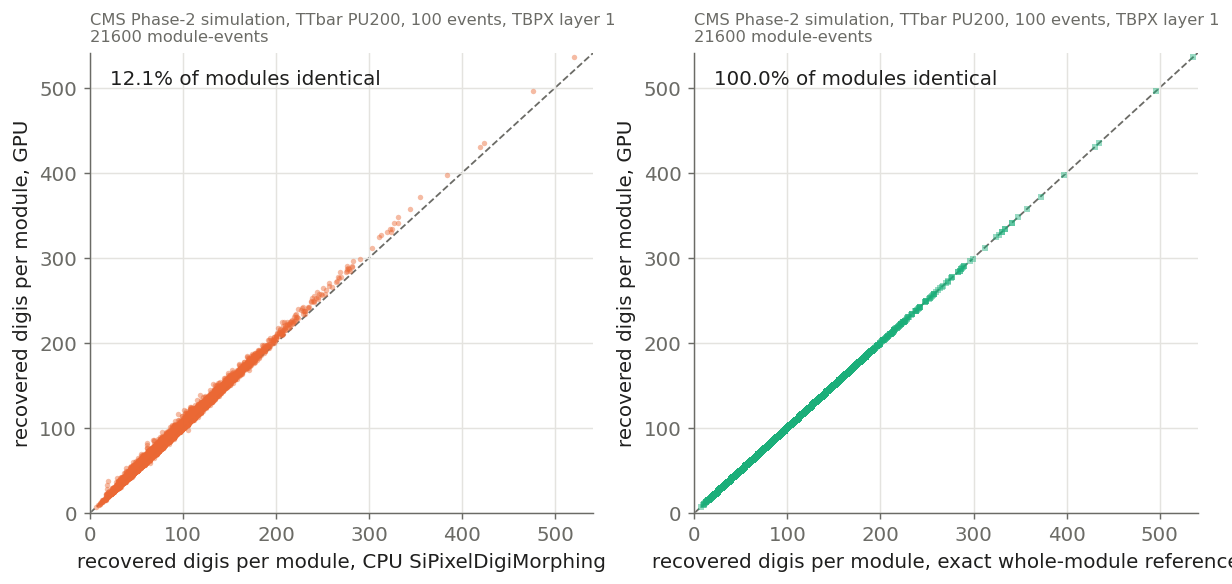
\includegraphics[width=0.84\textwidth]{recovered_digis_gpu_vs_cpu.png}
  \begin{columns}[T]
    \column{0.48\textwidth}
    \small vs CPU: 12.1\,\% of modules identical; 1\,630\,486 recovered pixels in common, 69\,844 differ
    \column{0.48\textwidth}
    \small vs exact: \HL{\textbf{100\,\% identical}}, 1\,696\,444 = 1\,696\,444, \textbf{0 differences}
  \end{columns}
\end{frame}

\begin{frame}{Where GPU and CPU differ: all CPU artefacts or the edge rule}
  \centering
  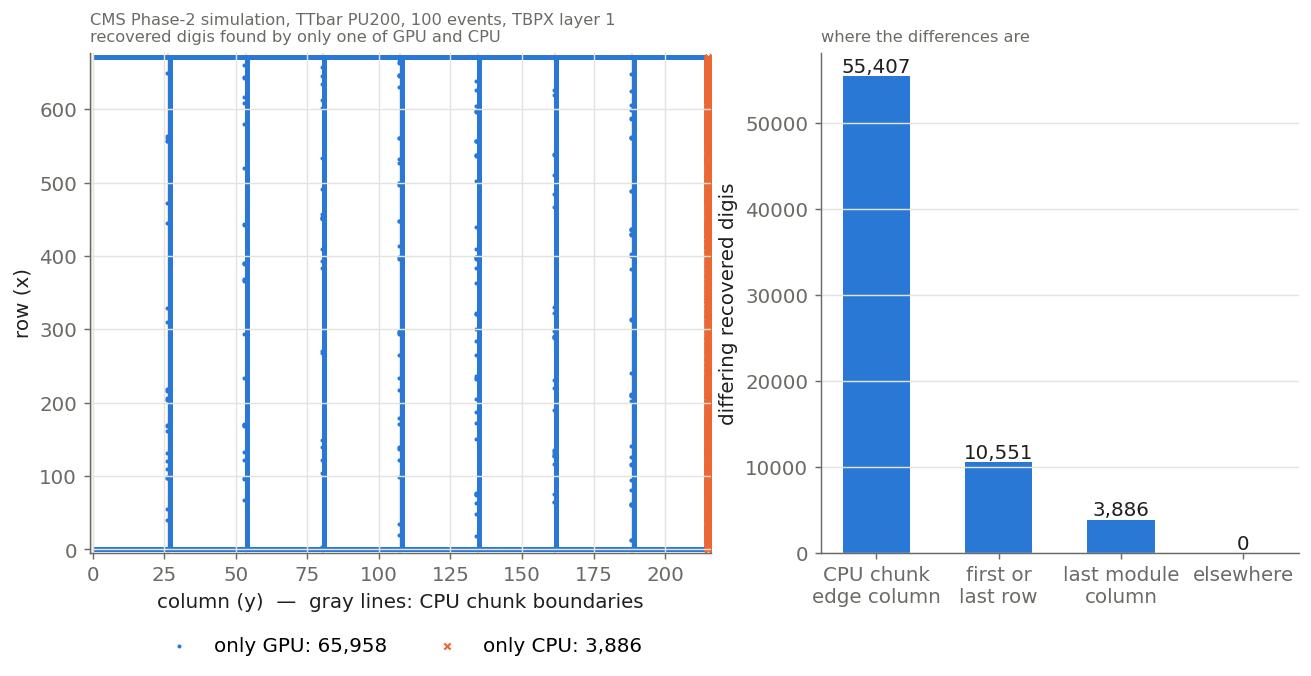
\includegraphics[width=0.66\textwidth]{difference_location.png}
  \begin{itemize}\small
    \item \textbf{55\,407} on the CPU's 27-column chunk edges: CPU does not dilate its 1-column halo (the halo = 1 bug)
    \item \textbf{10\,551} on the first/last row: deliberate Phase-1 GPU rule (beyond a row edge counts as filled)
    \item \textbf{3\,886} CPU-only on the last module column; \textbf{0 elsewhere}. In all 69\,844 the GPU agrees with the exact reference.
  \end{itemize}
\end{frame}

\begin{frame}{What morphing does: a broken track in TBPX L1}
  \centering
  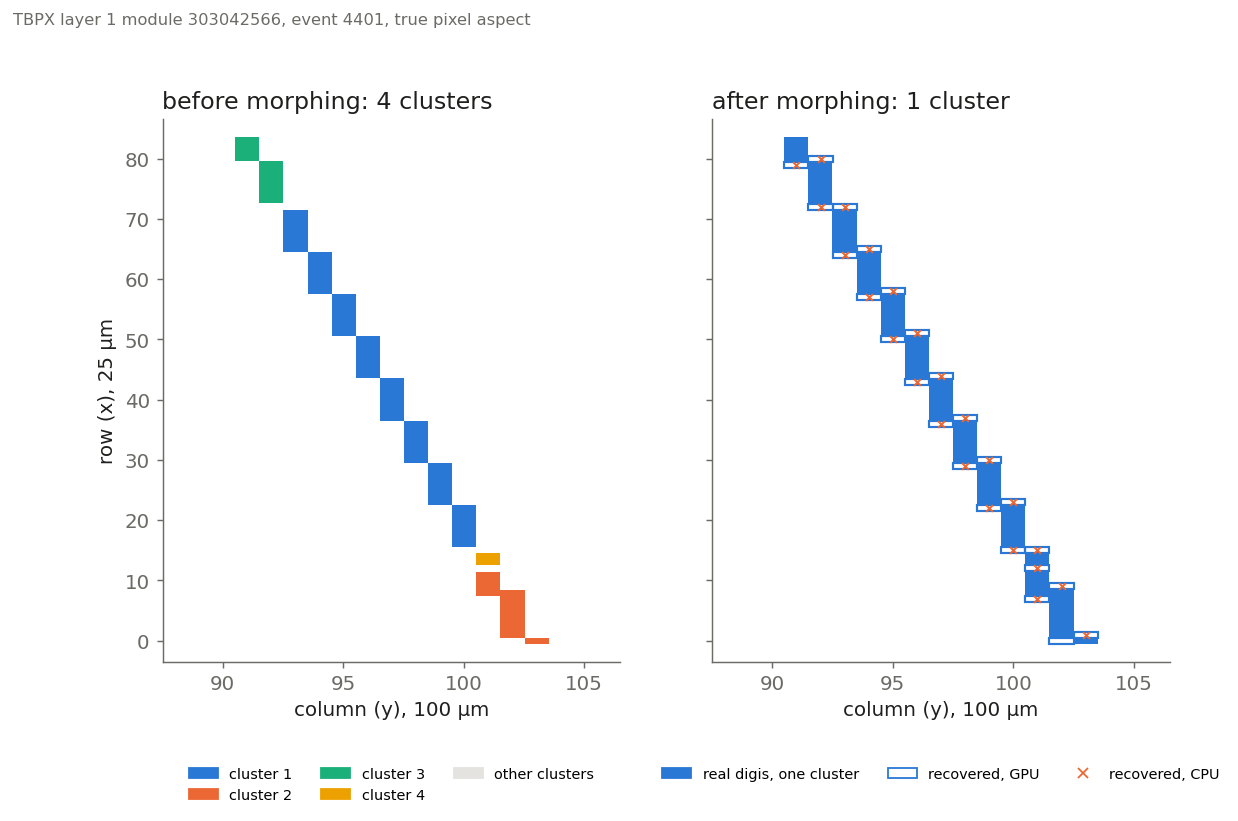
\includegraphics[height=0.70\textheight]{display_1.png}
  \takeaway{4 clusters $\to$ 1; GPU (boxes) and CPU (crosses) recover the same pixels here.}
\end{frame}

\begin{frame}{Effect on digis and clusters in TBPX L1}
  \begin{columns}[T]
    \column{0.36\textwidth}
    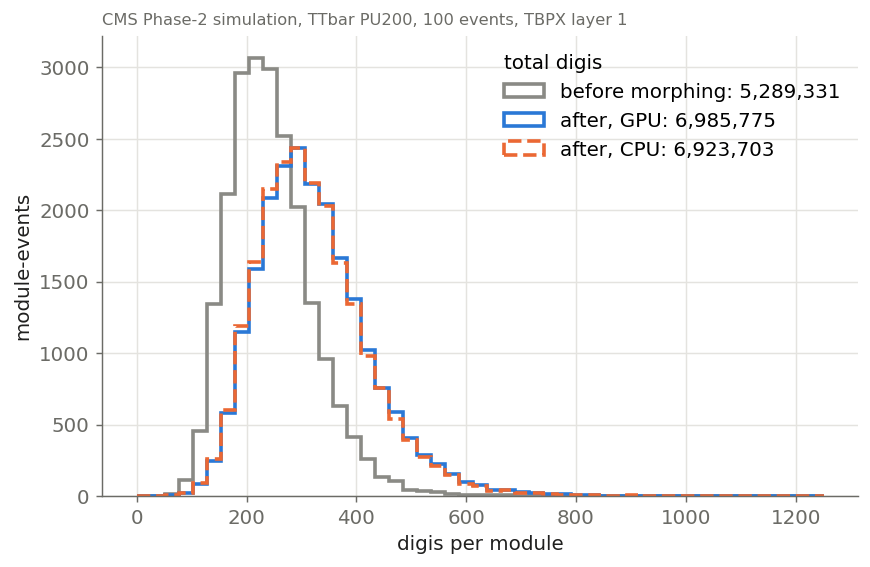
\includegraphics[height=0.37\textheight]{digis_per_module.png}\\[2pt]
    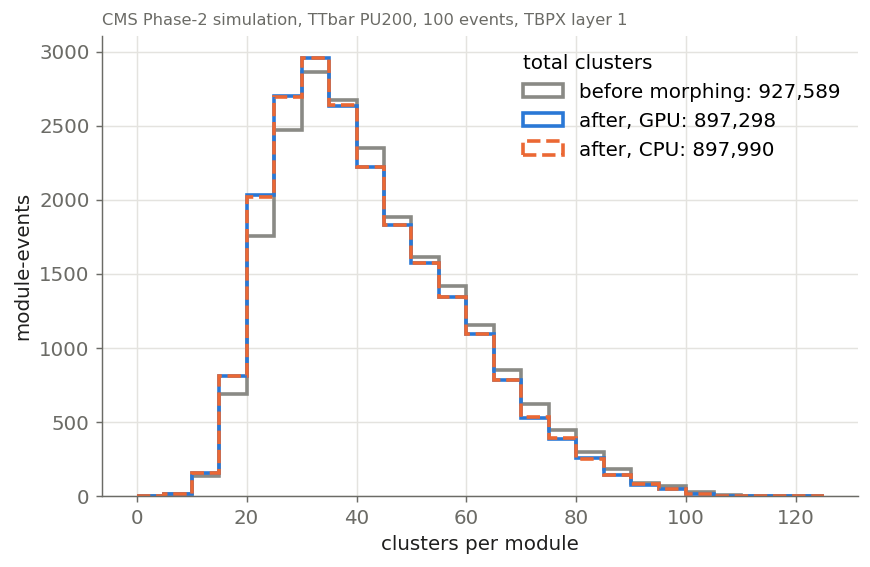
\includegraphics[height=0.37\textheight]{clusters_per_module.png}
    \column{0.60\textwidth}
    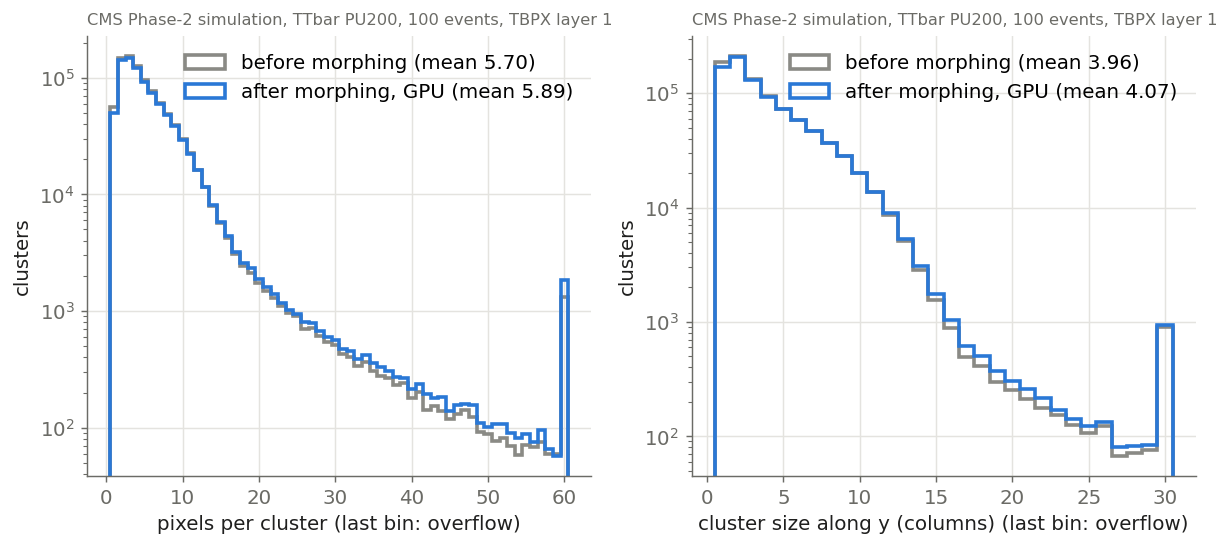
\includegraphics[width=\textwidth]{cluster_size_L1.png}
    \vspace{2pt}
    \begin{center}\small
    \begin{tabular}{@{}lrr@{}}
      \toprule
      & before & after (GPU) \\
      \midrule
      clusters & 927\,589 & 897\,298 (\textbf{$-$3.3\,\%}) \\
      clusters, CPU morphing & & 897\,990 \\
      mean pixels / cluster & 5.70 & 5.89 \\
      mean size in $y$ & 3.96 & 4.07 \\
      recovered / real digis & & +32\,\% \\
      \bottomrule
    \end{tabular}
    \end{center}
  \end{columns}
\end{frame}

\begin{frame}{A caveat: crossing clusters get merged}
  \begin{columns}[T]
    \column{0.62\textwidth}
    \includegraphics[width=\textwidth]{display_3_crop.png}
    \column{0.36\textwidth}
    \begin{itemize}
      \item A short cluster crossing a long one is \con{merged into it}
      \item Same behaviour on CPU (crosses) and GPU (boxes): it is the algorithm, not the port
      \item Closing bridges gaps of up to 2 pixels
      \item \textbf{To check} before enabling: hit resolution (CPE) and track efficiency / fake rate
    \end{itemize}
  \end{columns}
\end{frame}

\begin{frame}{Morphing off = master, bit for bit}
  \vspace{4pt}
  \begin{center}
  \begin{tabular}{@{}lr@{}}
    \toprule
    Check (100 PU200 events, T4) & Result \\
    \midrule
    stock config, this branch vs pristine \code{CMSSW\_20\_1\_X\_2026-10-20-2300} & \HL{\textbf{100 / 100 events identical}} \\
    digis compared (cluster index, charge, module) & 56\,142\,094 \\
    morphing off: GPU clusters vs 8-neighbour reference & 0 modules differ \\
    morphing on: clusters changed outside TBPX L1 & 0 \\
    \bottomrule
  \end{tabular}
  \end{center}
  \vspace{6pt}
  \begin{itemize}
    \item Default is \textbf{off}: nothing changes for existing Phase-2 workflows
    \item \con{Not yet checked}: Phase-1 (Run 3) output with the shared kernel code; same shared memory as master (38\,200\,B), but needs a Run-3 workflow comparison before a PR
  \end{itemize}
\end{frame}

% ===================================================================
\section{Configuration and code changes}
\begin{frame}[fragile]{What can be configured}
  \vspace{2pt}
  \begin{center}\small
  \begin{tabular}{@{}>{\raggedright\arraybackslash}p{0.30\textwidth}>{\raggedright\arraybackslash}p{0.17\textwidth}>{\raggedright\arraybackslash}p{0.47\textwidth}@{}}
    \toprule
    Parameter & Default & Meaning \\
    \midrule
    \code{DoDigiMorphing} & \code{False} & switch \\
    \code{MaxFakesInModule} & 1000 & recovered pixels per module; must be $<$ \code{maxPixInModule} (6000); real pixels capped at $6000-1000$ in morphing modules \\
    \code{barrelRegions} & \code{["1,1-99,1-99"]} & \code{"layer,ladder,module"}, ranges \code{A-B}; default = TBPX L1 (216 modules) \\
    \code{endcapRegions} & \code{[]} & \code{"disk,blade,side,panel"}; meaning for TFPX/TEPX detids \con{still to check} \\
    \midrule
    \multicolumn{3}{@{}l}{\textit{compile time, \code{::pixelClustering::phase2Morphing}:}} \\
    \code{stripCols} / \code{halo} & 44 / 2 & strip width and halo (buffer = 48 columns) \\
    \code{maxRows} & 1376 & largest module (1354 rows) rounded up to a word \\
    \bottomrule
  \end{tabular}
  \end{center}
\begin{lstlisting}[language=Python]
process.siPixelClustersPreSplittingAlpaka.DoDigiMorphing = True
process.siPixelClustersPreSplittingAlpaka.barrelRegions = ["1,1-99,1-99"]   # TBPX L1
\end{lstlisting}
\end{frame}

\begin{frame}{Files added and changed (\code{RecoLocalTracker/SiPixelClusterizer/plugins/alpaka/})}
  \vspace{2pt}
  \begin{center}\footnotesize
  \begin{tabular}{@{}>{\raggedright\arraybackslash}p{0.36\textwidth}r>{\raggedright\arraybackslash}p{0.50\textwidth}@{}}
    \toprule
    File & $+$/$-$ & What \\
    \midrule
    \code{PixelClustering.h} & 212/21 & strip morphing in \code{FindClus}; \code{morphingModuleIndex}; shared \code{image}/\code{temp}; \code{firstFake}, \code{maxPixels} \\
    \code{SiPixelMorphingConfig.h} & 35/0 & new namespace \code{::pixelClustering::phase2Morphing}: strip constants, \code{packSize} \\
    \code{SiPixelMorphingRegions.h} & \pos{new} 105 & \code{parseRegions}, \code{skipDetId}, moved out of \code{SiPixelRawToCluster.cc} \\
    \code{SiPixelPhase2DigiToCluster.cc} & 98/2 & 4 parameters; modules + sizes from geometry in \code{beginRun}; device copy \\
    \code{SiPixelRawToCluster.cc} & 6/91 & Phase 1: uses the shared header (pure move) \\
    \code{SiPixelRawToClusterKernel.dev.cc} & 21/8 & Phase-2 launch: morphing block size, fakes per morphing module \\
    \code{SiPixelRawToClusterKernel.h} & 4/1 & \code{makePhase2ClustersAsync} signature \\
    \code{../../test/alpaka/}\newline\code{testPhase2DigiMorphing.dev.cc} & \pos{new} 306 & unit test vs whole-module host reference \\
    \code{../../test/BuildFile.xml} & 10/0 & registers the test for all Alpaka backends \\
    \bottomrule
  \end{tabular}
  \end{center}
  {\footnotesize Not changed: \code{SimplePixelTopology.h}, the Phase-1 morphing logic, any \code{\_cff.py}. The validation-only commit is \textbf{not} pushed.}
\end{frame}

\begin{frame}{Why a new namespace and a new header}
  \begin{columns}[T]
    \column{0.49\textwidth}
    \textbf{\code{::pixelClustering::phase2Morphing}} in \code{SiPixelMorphingConfig.h}
    \begin{itemize}\small
      \item needed by \textbf{both} the host producer (size check, \code{packSize}, default \code{MaxFakesInModule}) and the kernel (strip layout)
      \item header already included by both; outside the Alpaka backend namespace, so host code can use it
      \item next to the existing \code{::pixelClustering} constants (\code{invalidModuleId}, ...)
      \item separate from Phase-1 \code{pixelStatus}, whose 160$\times$416 layout is \code{constexpr} and stays untouched
      \item a \code{static\_assert} keeps the strip buffer within the Phase-1 size
    \end{itemize}
    \column{0.49\textwidth}
    \textbf{\code{SiPixelMorphingRegions.h}} (namespace \code{siPixelMorphing})
    \begin{itemize}\small
      \item \code{parseRegions}/\code{skipDetId} were private members of the Phase-1 \code{SiPixelRawToCluster}
      \item Phase 2 needs exactly the same region syntax and selection
      \item moved, not copied: one implementation for both producers (91 lines removed from Phase 1)
      \item host-only (boost, \code{TrackerTopology}): kept out of the device headers
      \item Phase-1 behaviour unchanged
    \end{itemize}
  \end{columns}
\end{frame}

\begin{frame}{Summary and next steps}
  \begin{columns}[T]
    \column{0.50\textwidth}
    \textbf{Done}
    \begin{itemize}\small
      \item Phase-2 digi morphing in the Alpaka clusterizer: Run-3 bit logic on \textbf{44-column strips}, any module size up to 1376 rows
      \item No extra shared memory, same block size as master
      \item GPU = exact reference in \textbf{every} L1 module, 100 PU200 events
      \item All GPU--CPU differences explained (CPU halo bug, row-edge rule)
      \item Off = master, bit for bit; default off
    \end{itemize}
    \column{0.47\textwidth}
    \textbf{To do before a PR}
    \begin{itemize}\small
      \item Run-3 regression: Phase-1 output with the shared code
      \item Timing of \code{FindClus}, morphing on vs off
      \item ROCm run
      \item Endcap regions for TFPX/TEPX
      \item Era modifier / \code{HLT\_75e33} switch (none yet)
    \end{itemize}
    \textbf{Physics questions}
    \begin{itemize}\small
      \item crossing clusters merged: CPE and tracking impact
      \item which regions to enable (L1 only?) once thresholds and irradiation are simulated
    \end{itemize}
  \end{columns}
\end{frame}

\begin{frame}[fragile]{The full change: \code{git diff -{}-stat a19318d617f phase2-digimorphing}}
\begin{lstlisting}[language={},basicstyle=\ttfamily\scriptsize,keywordstyle={}]
 .../SiPixelClusterizer/plugins/alpaka/PixelClustering.h         | 233 +++++++++++++++++++--
 .../SiPixelClusterizer/plugins/alpaka/SiPixelMorphingConfig.h   |  35 ++++
 .../SiPixelClusterizer/plugins/alpaka/SiPixelMorphingRegions.h  | 105 ++++++++++
 .../plugins/alpaka/SiPixelPhase2DigiToCluster.cc                | 100 ++++++++-
 .../SiPixelClusterizer/plugins/alpaka/SiPixelRawToCluster.cc    |  97 +--------
 .../plugins/alpaka/SiPixelRawToClusterKernel.dev.cc             |  29 ++-
 .../plugins/alpaka/SiPixelRawToClusterKernel.h                  |   5 +-
 RecoLocalTracker/SiPixelClusterizer/test/BuildFile.xml          |  10 +
 .../test/alpaka/testPhase2DigiMorphing.dev.cc                   | 306 ++++++++++++++++++++++++++++
 9 files changed, 797 insertions(+), 123 deletions(-)
\end{lstlisting}
  \begin{itemize}\small
    \item Base: \code{a19318d617f} (merge of cms-sw/cmssw\#52208) in \code{CMSSW\_20\_1\_X\_2026-10-20-2300}
    \item Commits: \code{15e2048e532} ``Phase-2 digi morphing in the Alpaka pixel clusterizer'', \code{7dd02b835e3} ``allow modules with up to 1376 rows (big pixels)''
    \item Without the moved region code and the test: $\approx$\,380 added lines, comments included
    \item \href{https://github.com/Chirayu18/cmssw/compare/a19318d617ffe6d96535142b12027d5d50cc08c3...phase2-digimorphing}{\color{cmsblue}github.com/Chirayu18/cmssw/compare/\ldots phase2-digimorphing}
  \end{itemize}
\end{frame}

% ===================================================================
\appendix
\begin{frame}
  \centering\vfill{\color{cmsblue}\Large\bfseries Backup}\vfill
\end{frame}

\begin{frame}{More event displays}
  \begin{columns}[T]
    \column{0.49\textwidth}
    \includegraphics[width=\textwidth]{display_2_crop.png}
    \column{0.49\textwidth}
    \includegraphics[width=\textwidth]{display_4_crop.png}
  \end{columns}
  \vspace{4pt}
  {\small Real digis coloured by cluster before morphing (left of each), merged cluster after (right); GPU recovered = boxes, CPU recovered = crosses. True 25$\times$100\,\textmu m aspect.}
\end{frame}

\begin{frame}{Recovered pixels per module: GPU minus CPU}
  \centering
  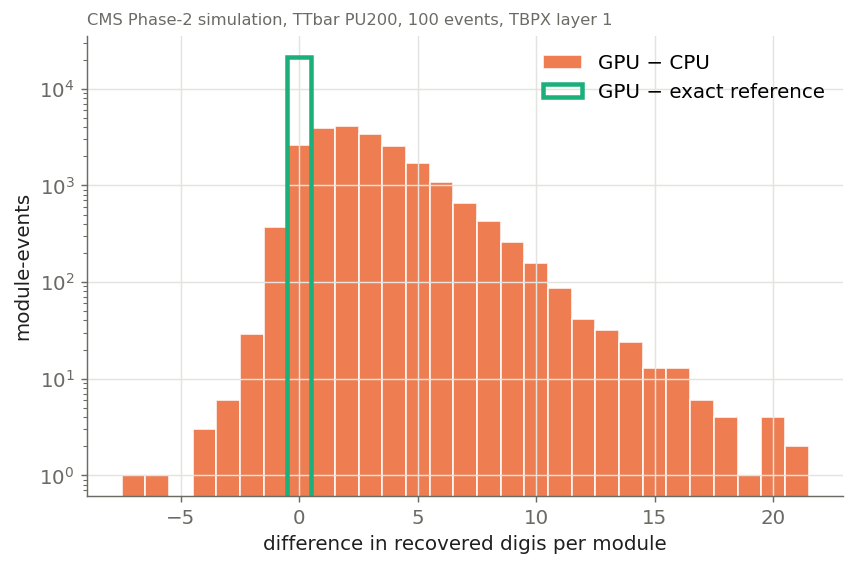
\includegraphics[width=0.62\textwidth]{recovered_digis_difference.png}
  \vspace{4pt}

  {\small GPU recovers more, because the CPU misses the pixels at its own chunk edges.}
\end{frame}

\begin{frame}{Validation numbers (\code{summary.json})}
  \vspace{4pt}
  \begin{center}\small
  \begin{tabular}{@{}lr@{\hspace{2em}}lr@{}}
    \toprule
    real digis, L1 & 5\,289\,331 & diff.\ pixels GPU vs CPU & 69\,844 \\
    recovered, GPU & 1\,696\,444 & \quad only GPU & 65\,958 \\
    recovered, exact reference & 1\,696\,444 & \quad only CPU & 3\,886 \\
    recovered, CPU & 1\,634\,372 & \quad at CPU chunk edge & 55\,407 \\
    recovered, both & 1\,630\,486 & \quad first/last row & 10\,551 \\
    max recovered in a module & 536 & \quad last column (CPU only) & 3\,886 \\
    recovered outside L1 & 0 & \quad elsewhere & 0 \\
    clusters before / GPU / CPU & 927\,589 / 897\,298 / 897\,990 & GPU side = exact ref. & 69\,844 / 69\,844 \\
    \bottomrule
  \end{tabular}
  \end{center}
  {\small Plots and numbers: \code{/eos/user/c/cgupta/phase2morph/plots/}. Config and analyzer: \code{UserCode/Phase2MorphValidation} (validation-only commit \code{7e7e9e8fac9}).}
\end{frame}

\begin{frame}{Register limit on the T4, in detail}
  \begin{columns}[T]
    \column{0.55\textwidth}
    \begin{itemize}\small
      \item \code{FindClus}, Phase 2, sm\_75: 143 registers/thread
      \item driver reports \code{maxThreadsPerBlock} = \textbf{384} for this kernel
      \item a plain $65\,536 / (32\times144)$ estimate gives 14 warps (448); the lower limit is likely the per-quarter split of the register file (16k per SM sub-partition): \textit{inferred, not measured}
      \item 448 threads (histogram 6000 + 2400) $\to$ \code{cudaErrorLaunchOutOfResources}
    \end{itemize}
    \column{0.42\textwidth}
    \textbf{How it was measured}
    \begin{itemize}\small
      \item \code{cuobjdump -res-usage}: registers, shared memory
      \item \code{cudaFuncGetAttributes}: \code{maxThreadsPerBlock} = 384
      \item \code{compute-sanitizer}: 0 errors
      \item the SerialSync backend passed in both failing cases
    \end{itemize}
  \end{columns}
\end{frame}

\begin{frame}{References}
  \small
  \begin{itemize}
    \item Tracker DPG workshop, 14--16 Oct 2026, \href{https://indico.cern.ch/event/1707530}{\color{cmsblue}indico.cern.ch/event/1707530}: talks by A.~Bocci (Alpaka), N.~Bartosik (geometry), G.~Mersi (IT data formats), M.~Magherini (IT calibration), S.~Dutta (Phase-2 digitizer), M.~Musich (HLT tracker reco), J.~Schulz / M.~Grutta (HLT tracking), Run-3 pixel experience
    \item Phase-1 GPU morphing: \code{RecoLocalTracker/SiPixelClusterizer/plugins/alpaka/PixelClustering.h} (cms-sw/cmssw master)
    \item CPU morphing: \code{RecoLocalTracker/SiPixelDigiReProducers/plugins/SiPixelDigiMorphing.cc}
    \item This work: \href{https://github.com/Chirayu18/cmssw/compare/a19318d617ffe6d96535142b12027d5d50cc08c3...phase2-digimorphing}{\color{cmsblue}Chirayu18/cmssw, branch \code{phase2-digimorphing}}
  \end{itemize}
\end{frame}

\end{document}
